\documentclass[manuscript=suppinfo,email=true, hyperref=true, keywords=false]{achemso}
\usepackage[utf8]{inputenc}
\usepackage{graphicx}
\usepackage{tabularx}
\usepackage{amsmath}
\usepackage{times}
\usepackage{todonotes}
\newcommand{\Fig}{Fig.}
\renewcommand{\thesection}{S\arabic{section}}
\renewcommand{\theequation}{S\arabic{equation}}
\SectionNumbersOn
\usepackage{xr-hyper}
\usepackage{xcolor}
\externaldocument[main-]{paper}

% \usepackage{lineno}
% \linenumbers

\author{Roman M. Wyss} \affiliation{Soft Materials,
  Department of Materials, Eidgenössische Technische
  Hochschule (ETH) Zürich, Vladimir-Prelog-Weg 1-5, Zürich CH-8093,
  Switzerland.  }
\altaffiliation{R. M. W. and T. T. contributed equally to this work}
\author{Tian Tian} \affiliation{Institute for
  Chemical and Bioengineering Department of Chemistry and Applied
  Biosciences, Eidgenössische Technische Hochschule (ETH) Zürich,
  Vladimir-Prelog-Weg 1-5, Zürich CH-8093, Switzerland.}
\altaffiliation{R. M. W. and T. T. contributed equally to this work}

\author{Khadija Yazda} \affiliation{Nanoscience for Energy Technology and Sustainability,
Department of Mechanical and Process Engineering,
Eidgenössische Technische Hochschule (ETH) Zürich,
Tannenstrasse 3, Zürich CH-8092, Switzerland.}

\author{Hyung Gyu Park} \affiliation{Nanoscience for Energy Technology and Sustainability,
Department of Mechanical and Process Engineering,
Eidgenössische Technische Hochschule (ETH) Zürich,
Tannenstrasse 3, Zürich CH-8092, Switzerland.}
\alsoaffiliation{Mechanical Engineering, Pohang University of Science and
  Technology (POSTECH), 77 Cheongam-ro, Nam-gu, Pohang, Gyeongbuk,
  Republic of Korea.}
\email{iduserpark@gmail.com}

\author{Chih-Jen Shih}  \affiliation{Institute for
  Chemical and Bioengineering Department of Chemistry and Applied
  Biosciences, Eidgenössische Technische Hochschule (ETH) Zürich,
  Vladimir-Prelog-Weg 1-5, Zürich CH-8093, Switzerland.}
\email{chih-jen.shih@chem.ethz.ch}

\title{Macroscopic Salt Rejection through Electrostatically Gated Nanoporous Graphene}

%%%%%%%%%%%%%%%%%%%%
%Main
%%%%%%%%%%%%%%%%%%%%
\begin{document}

%%%%%%%%%%%%%%%%%%%%%%%%%%%%%%
% Main text
%%%%%%%%%%%%%%%%%%%%%%%%%%%%%%
\clearpage{}

\section{Graphene membrane manufacturing and results.}
\label{sec:exp}

\begin{figure}[htbp]
  \centering
  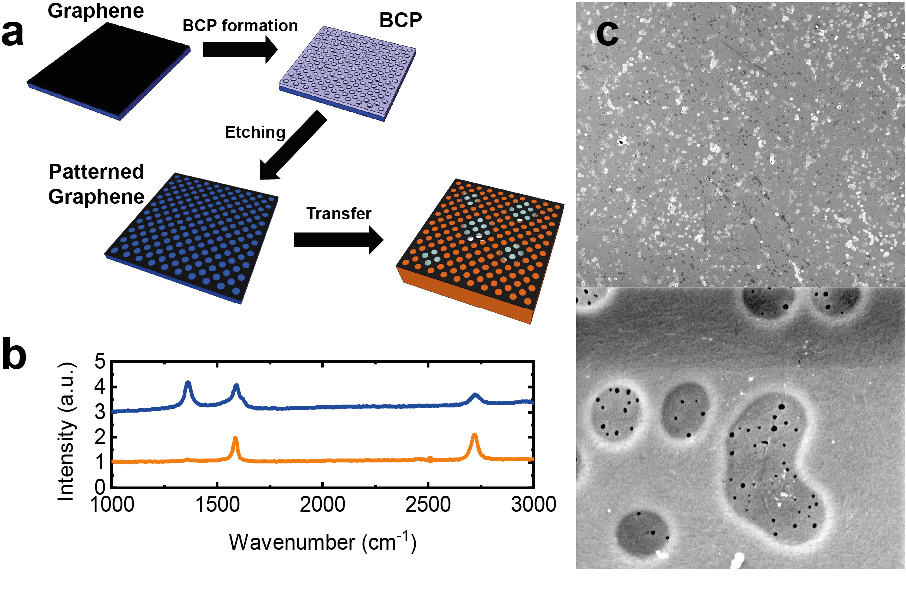
\includegraphics[width=0.95\linewidth]{img/SI-1.png}
  \caption{\textbf{a}. Schematic of manufacturing process for
    patterning of double layer graphene. Graphene is synthesized and
    transferred to a substrate (glass slide) to yield a double
    layer. s-BCP is spin-coated and annealed in vacuum to undergo microphase
    separation, followed by plasma etch and wet etching yielding a
    porous polystyrene (PS) mask. Anisotropic etching of the mask
    leads to patterning the underlying graphene, PS is removed by
    thermal annealing. The porous graphene is then transferred to a
    substrate (e.g. PCTE). \textbf{b}. Raman spectra of graphene
    before (orange curve) and after (blue
    curve) patterning. An increase of the D-peak at 1350 cm$^{-1}$ indicates the
    formation of defects and edges. The spectra have been normalized
    to the G-peak intensity and offset for better
    comparison. \textbf{c}. SEM graph of patterned graphene on PCTE at
    lower (top) and higher (bottom) magnifications.
    % Note that tears in
    % graphene appear bright white with a black center.
  }
  \label{fig:exp}
\end{figure}

\section{Ion diffusion measurement and calculation}
\label{sec:measure}

The ion diffusion through b-PCTE has been performed using a sample
sandwiched between two layers of Aluminum tape where the edges have
been sealed using water-resistant epoxy (ACS Marine Epoxy) to avoid
interlayer leakage pathways \cite{Choi_2018}.  The sample was inserted in
the fixture following the same wetting procedure described in the main
text Methods and was kept wet for the entire series of experiments.

\begin{table}[htbp]
  \centering
  \begin{tabular}{lc}
    \hline
    Salt & $D$ (10$^{9}$ m$^{2}\cdot$s$^{-1}$) \\
    \hline
    K$^{+}$     & 1.95 \\
    Na$^{+}$    & 1.33 \\
    Li$^{+}$    & 1.03 \\
    SO$_{4}^{2-}$       & 1.06 \\
    Ca$^{2+}$   & 0.79\\
    Mg$^{2+}$ & 0.7\\
    Fe{[(CN)$_{6}$]}$^{3-}$   & 0.90\\
    Cl$^{-}$ &  2.03 \\
               \hline
  \end{tabular}
  \caption{Different diffusivities for the anions and cations of the
    salts used in this work \cite{vanysek_2000}. The theoretical
    diffusion through PCTE can be calculated using Eq. 1 in the main
    text and the diffusivities of the respective anion and cation.}
  \label{tab:diff}
\end{table}

The conductivity increase $s$ (mS$\cdot$cm$^{-1}\cdot$d$^{-1}$) is
converted into ion permeation rates $\boldsymbol{J}_{\mathrm{PCTE}}$
(mol$\cdot$m$^{-2}\cdot$s$^{-1}$) by use of a calibration factor
$c_{\mathrm{f}}$, the volume of LCR ($V_{\mathrm{LCR}}$) , the area of
the membrane $A$ and the time $t$ as:
\begin{equation}
  \label{eq:JPCTE}
  \boldsymbol{J}_{\mathrm{PCTE}} = \frac{s V_{\mathrm{LCR}}}{c_{\mathrm{f}} A t}
\end{equation}
The calibration factors for all salts have been obtained by a linear
fit of conductivity \textit{versus} concentration for 4 solutions with
concentrations from 10$^{-4}$ M to 10$^{-2}$ M and extracting the
resulting slope. The rest of the factors are $V_{\mathrm{LCR}}$ = 7.33
mL, $A$ = 9$\times$10$^{-6}$ m$^{-2}$. Table \ref{tab:exp-2} shows the
averaged conductivity increase s, the extracted calibration factors
$c_{\mathrm{f}}$ and the resulting ion permeation rates using
Eq. \ref{eq:JPCTE}. The values from this table are shown in main text \Fig 2b
(blue bars).
\begin{table}[htbp]
  \centering
  \begin{tabular}{lccc}
    \hline
    Salt & $s$ (mS$\cdot$cm$^{-1}$d$^{-1}$) & $c_{\mathrm{f}}$ (mS$\cdot$cm$^{-1}\cdot$mol$^{-1}\cdot$L) &
                                                                                                            $\boldsymbol{J}_{\mathrm{PCTE}}$ (10$^{6}$ mol$\cdot$m$^{-2}\cdot$s$^{-1}$)\\
    \hline
    KCl & 1.51$\pm$0.27$\times$10$^{-2}$  & 106   & 1.34 $\pm$ 0.24\\
    NaCl        & 9.90$\pm$0.17$\times$10$^{-3}$ & 91    & 1.02 $\pm$ 0.02\\
    LiCl        & 6.03 $\pm$0.80$\times$10$^{-3}$        & 83    & 0.682 $\pm$ 0.090\\
    CaCl$_{2}$  & 1.25$\pm$0.1$\times$10$^{-2}$    & 149   & 0.789 $\pm$ 0.063\\
    MgSO$_{4}$  & 8.80$\pm$1.2$\times$10$^{-3}$   & 130   & 0.633 $\pm$ 0.084\\
    K$_{3}$[Fe(CN)$_{6}]$ & 2.40$\pm$0.28$\times$10$^{-2}$   & 395   & 0.575 $\pm$ 0.063\\
    K$_{2}$SO4$_{4}$    & 1.98$\pm$0.20$\times$10$^{-2}$  & 258   & 0.722 $\pm$ 0.073\\
    \hline
  \end{tabular}
  \caption{Extracted slope $s$ as an averaged result from 3 consecutive
    measurements, the calibration factors $c_{\mathrm{f}}$ and the resulting ion
    permeation $\boldsymbol{J}_{\mathrm{PCTE}}$ through b-PCTE membranes for all salts.}
  \label{tab:exp-2}
\end{table}

The experimentally observed flux reduction through PG-PCTE upon
gating, $\eta$, for all the salts studied here (with concentration of
0.1 mM in HCR), can be found in \Fig{} \ref{fig:eta-all}. The effective salt
rejection ratio $\xi$ is then extracted using main text
Eq. \ref{main-eq:xi-def}.

\begin{figure}[htbp]
  \centering
  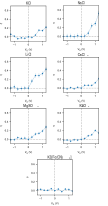
\includegraphics[width=0.5\linewidth]{img/SI-eta-all.pdf}
  \caption{Measured $\eta$ values as function of $V_{\mathrm{G}}$ for
    different salts used in this work. The concentration in HCR is 0.1
    mM in all cases.}
  \label{fig:eta-all}
\end{figure}


\section{Control experiment with copper tape}
\label{sec:copper}
We make sure that the applied voltage is effectively applied via the
graphene membrane and not through leakage directly coupling the
copper tape to the ionic solution. For this, we use a device as in \Fig
1a, omitting the graphene and measuring the current through the
membrane with the Autolab electrochemical workstation using the
membrane as working electrode and a platinum wire as counter/reference
electrode 3.5 cm apart in 0.1 mM KCl. When no graphene is inserted in
the device, a current in the baseline range ($\sim$ 0.1 nA) is
observed, indicating no current passing from the membrane. However, if
graphene is inserted, a current in the range of $\sim$ 10 - 100 nA is
measured. If the copper tape is in contact with the solution when
omitting the Kapton tape, the current increases to $\sim$ 1 - 10
$\mathrm{\mu}$A, independent of the exposed area of the copper tape to
the solution.

% \pagebreak

\section{Circuit analog model of transport through PG-PCTE}
\label{sec:R-model}

\begin{figure}[htbp]
  \centering
  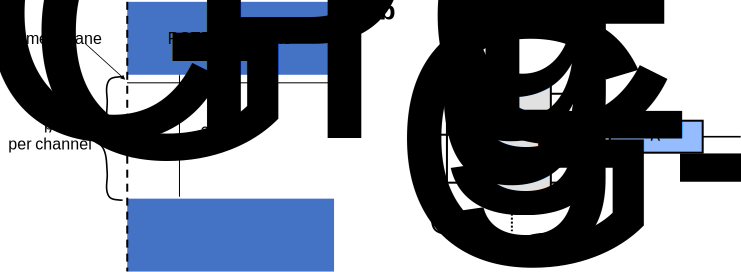
\includegraphics[width=0.8\linewidth]{img/SI-resistance-rectification.pdf}
  \caption{Simple circuit analog model for the transport through
    PG-PCTE membrane. \textbf{a}. Schematic of PG-PCTE membrane in
    cross-section view. \textbf{b}. Model for transport resistance in
    analogy to an electric circuit. This schematic depicts a cut
    through a PG-PCTE membrane showing a single PCTE pore and multiple
    graphene pores.}
  \label{fig:R-model}
\end{figure}
The ionic transport through the PG-PCTE membrane is the concerted
effect the transport resistance through PG and PCTE membranes,
respectively. As schematically shown in \Fig{} \ref{fig:R-model}, the
overall transport resistance of the system is composed of the series
resistance $R_{\mathrm{G}}$ and $R_{\mathrm{PCTE}}$, respectively. For
both PG and PCTE membranes, the resistance $R$ is defined as the ratio
between the concentration between HCR and LCR $\Delta c$, and the total diffusive current $I$ as:
\begin{equation}
\label{eq:1}
R_{i} = \Bigg|\frac{\Delta c}{I_{i}}\Bigg| =  \Bigg|\frac{\Delta c}{J_{i}A_{i}}\Bigg|
\end{equation}
where $i$ denotes the membrane type and $A_{i}$ is the area of the
pore. We further treat $R_{\mathrm{G}}$ as the effective resistance of
$\gamma$ parallel resistors with individual resistance
$R_{\mathrm{g}}$, where $\gamma$ is the average number of PG pores per
PCTE channel, and $R_{\mathrm{g}}$ is the average transport resistance
per PG pore. The value of $\gamma$ is determined from geometric
analysis of both membranes: given the pore number density of PG
($\sim$1.25$\times$10$^{14}$ m$^{-2}$), the pore number density of
PCTE ($\sim$1.50$\times$10$^{12}$ m$^{-2}$), and the percentage of
PCTE pores with PG on top ($\sim$0.13), $\gamma$ is determined to be
$\sim$10.83.

The objective of the circuit analog model is to find effective salt
rejection ratio through PG, $\xi$ extracted from the experimental
$\eta$ values (defined in main text Eq. \ref{main-eq:rejection}). By
defining $R_{\mathrm{G}}^{0}=R_{\mathrm{G}}(V_{\mathrm{G}}=0)$,
$\delta = R_{\mathrm{PCTE}} / R_{\mathrm{G}}^{0}$,
$\chi = R_{\mathrm{G}}/R_{\mathrm{G}}^{0}$, $\eta$ is rewritten using
transport resistances as:
\begin{equation}
  \begin{aligned}[t]
      \label{eq:eta-R}
  \eta &= 1 - {\displaystyle
    \frac{(R_{\mathrm{PCTE}} + R_{\mathrm{G}})^{-1}}
    {(R_{\mathrm{PCTE}} + R_{\mathrm{G}}^{0})}} \\
    &= 1 - \frac{\delta + 1}{\delta + R_{\mathrm{G}}/R_{\mathrm{G}}^{0}} \\
    &= 1 - \frac{\delta + 1}{\delta + \chi}
  \end{aligned}
\end{equation}
Consequentially, the
salt rejection ratio $\xi$, is associated with $\chi$ by
$\xi = 1 - \chi^{-1}$ and is related with $\delta$ and $\eta$ via:
\begin{equation}
  \label{eq:xi-deriv}
  \begin{aligned}[t]
    \xi &= 1 - \chi^{-1} \\
    &= \frac{(\delta + 1) \eta}{\delta\eta + 1}
  \end{aligned}
\end{equation}
which is main text Eq. \ref{main-eq:xi-def}. When $0<\eta<1$ (salt
rejection regime) and $\delta>0$, Eq. \ref{eq:xi-deriv} always
guarantees $\xi>\eta$, since $\delta + 1$ is always larger than
$\delta\eta + 1$. In other words, due to the existence of
$R_{\mathrm{PCTE}}$, the effective salt rejection through PG upon
gating, is always larger than that experimentally observed.

Next we seek the value of $\delta$, the resistance ratio
between the PCTE and PG membranes, without gating. The range
of $\delta$ can be estimated from experimental data in main text
\Fig{} \ref{main-fig:2}b using the relation:
\begin{equation}
  \label{eq:exp-delta}
  \delta = \left(\frac{\boldsymbol{J}_{\mathrm{PCTE}}}{\boldsymbol{J}_{\mathrm{PG}}^{0}} -1 \right)^{-1}
\end{equation}
by assuming the validity of the circuit analog model for all salt
systems. As shown in \Fig{} \ref{fig:delta-compare}, the
experimentally estimated value of $\delta$ varies from 1 to 5,
indicating that the resistance of the PG membrane is dominating in the
PG-PCTE system.
\begin{figure}[htbp]
  \centering
  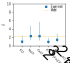
\includegraphics[width=0.55\linewidth]{img/SI-delta-estimate.pdf}
  \caption{Comparison between the $\delta$ value estimated from simple
    geometric model (Eq. \ref{eq:delta-resistance}) and from
    experimental value (Eq. \ref{eq:exp-delta}), showing good
    agreement between the two methods.  }
  \label{fig:delta-compare}
\end{figure}
$\delta$ can also be estimated using geometric parameters of both
membranes. For a long PCTE channel with length $L$ and
$r_{\mathrm{PCTE}}$, $R_{\mathrm{PCTE}}$ has power law of
$L/r_{\mathrm{PCTE}}^{2}$, while for a graphene pore
with radius $r_{\mathrm{G}}$ and vanishing thickness, the resistance of individual pore $R_{\mathrm{g}}^{0}$
has power law $1/r_{\mathrm{G}}$ \cite{O_Hern_2014}, which are expressed as:
\begin{subequations}
\begin{eqnarray}
  \label{eq:R-both}
  R_{\mathrm{PCTE}} &= &k_{\mathrm{PCTE}} \frac{L}{r_{\mathrm{PCTE}}^{2}} \\
  R_{\mathrm{g}}^{0} &= &k_{\mathrm{g}} \frac{1}{r_{\mathrm{G}}}
\end{eqnarray}
\end{subequations}
where $k_{\mathrm{PCTE}}$ and $k_{\mathrm{g}}$ are the coefficient
associated with PCTE and PG membranes, respectively. The value of
$\delta$ is then expressed as:
\begin{equation}
  \label{eq:delta-resistance}
  \delta
  = \frac{R_{\mathrm{PCTE}}}{R_{\mathrm{G}}^{0}}
  = {\displaystyle
    \frac{k_{\mathrm{PCTE}}}{k_{\mathrm{g}}}
    \frac{L r_{\mathrm{G}} \gamma}
        {r_{\mathrm{PCTE}}^{2}}}
\end{equation}
Here we take $L$=24 $\mu$m, $r_{\mathrm{G}}$=10 nm,
$r_{\mathrm{PCTE}}$=200 nm. From simple Fick's law\cite{Beers_2006},
the coefficient $k_{\mathrm{PCTE}}$ is determined as
$1/(D_{\mathrm{\pm}} \pi)$. On the other hand $k_{\mathrm{G}}$ varies
by the choice of model, ranging from $3 \pi / D_{\mathrm{\pm}}$ using
the analog of the Sampson formula for
fluid\cite{Roscoe_1949,Celebi_2014}, to $1/(2 D_{\mathrm{\pm}})$ from
the Hill formula for disk absorption model
\cite{Hill_1975,Grebenkov_2018}. As a result the theoretical value of
$\delta$ has lower bound of $\sim$2.2 (Sampson formula, orange line in
\Fig{} \ref{fig:delta-compare}) to $\sim$40.5 (Hill formula). We note
our experimental values of $\delta$ is in good agreement estimated
from the Sampson formula (which we use in the main text) while lower
than the Hill formula. Having a higher estimated value of $\delta$
could yield unreasonably high value of $\xi$ and the influence of
concentration is deviated from our theoretical predictions. Further
theoretical analysis taking nonidealities including surface adsorption
and chemical nature of pore edge, is required to have better
understanding of graphene's transport resistance.


% On the other hand, the transport through
% 2D pore with high radius/thickness ratio falls into the regime of the
% Sampson formula \cite{Roscoe_1949}, where the entrance resistance
% dominates over the bulk resistance, with the formula as
% \cite{Roscoe_1949,Celebi_2014}:
% \begin{equation}
%   \label{eq:sampson}
%   R_{\mathrm{g}}^{0} = \frac{1}{D} \frac{3 \pi}{r_{\mathrm{G}}}
% \end{equation}
% We therefore estimate the value of $\delta$ as:



\section{KCl Debye length and conductivity}
\label{sec:debye}
Table \ref{tab:debye} gives an overview about the measured
conductivities and their calculated Debye length values for KCl. The
information is used to plot the $\xi$ versus $c_{0}$ curve.

\begin{table}[htbp]
  \centering
  \begin{tabular}{lccc}
    \hline
    $c_{0}$ (mM) & Conductivity (mS$\cdot$cm$^{-1}$) & $\lambda_{\mathrm{D}}$ (nm)\\
    \hline
    0.1&        1.90$\times$10$^{-2}$ &        30.4\\
    0.33&       5.41$\times$10$^{-2}$ & 16.0\\
    1   &1.33$\times$10$^{-1}$ & 10.0\\
    3.3&     5.13$\times$10$^{-1}$ &  6.0\\
    10&      1.08    &3.3\\
    \hline
  \end{tabular}
  \caption{Conductivity and calculated Debye lengths of various KCl
    concentrations in order to obtain rectification versus
    concentration curves. }
  \label{tab:debye}
\end{table}

\section{Measurement of charge carrier density of patterned graphene}
\label{sec:charge-dens}
The intrinsic charge carrier density of graphene was measured using a
field electron transistor (FET) in air with a 300nm SiO$_2$ as a
gate. The device setup is shown in \Fig{} \ref{fig:charge-dens}a,
where the source and drain electrodes were deposited onto the PG
sample transferred onto 300nm SiO$_2$ on doped Silicon. The
characteristic drain-source current $I_{\mathrm{DS}}$ as a function of
$V_{\mathrm{G}}$ is shown in \Fig{} \ref{fig:charge-dens}. The
charge-neutral point gate voltage $V_{\mathrm{CNP}}$ is measured to be 2.8 V.
Using the capacitance of the SiO$_{2}$ dielectric, we an intrinsic
charge density of $\sim{}$1.4$\times$10$^{11}$
\textit{e}$\cdot$cm$^{-2}$, and a shift in the PG's Fermi level by
$\sim{}$48 meV, which is negligible compared with the gate-induced
charge density in our experiments. Therefore, the assumption that the
PG sample is intrinsic without gating, is justified.

\begin{figure}[htbp]
  \centering
  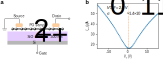
\includegraphics[width=0.8\linewidth]{img/SI-gr-transistor.pdf}
  \caption{Characterization of the intrinsic charge density of the PG
    sample using field effect transistor. \textbf{a}. The setup of the
    PG-FET. \textbf{b}. The I$_{\mathrm{DS}}$ as a function of
    $V_{\mathrm{G}}$. The charge neutral point gate voltage is
    determined as $\sim{}$2.8 V, corresponding to an intrinsic charge
    density of $\sim{}$1.4$\times$10$^{11}$
    \textit{e}$\cdot$cm$^{-2}$, which is negligible compared with the
    gate-induced charges.}
  \label{fig:charge-dens}
\end{figure}

\section{Effect of pore size distribution}
\label{sec:pore-dist}

One practical issue with large-area nanoporous graphene samples is
that the unavoidable large pores will act as preferred pathways for
the transported species and strongly attenuates the salt rejection
effect. In this section we provide a detailed discussion about the
influence of pore size distribution on the salt rejection through the
PG-PCTE membrane. As seen from main text \Fig{} \ref{main-fig:1}c
inset, the average distance between individual nanopores is larger
than the largest Debye length studied here ($\sim{}$ 30 nm for 1 mM 1:1
salt solution), we can assume that the ionic transport pathways
through different nanopores do not influence each other and the total
ionic flux $\boldsymbol{J}_{\mathrm{PG}}$ is the summation of fluxes
through individual pores $\boldsymbol{J}_{i}$:
\begin{equation}
\label{eq:J-total}
\boldsymbol{J}_{\mathrm{PG}} = \sum_{i} \boldsymbol{J}_{i} = \sum_{r_{i}} x_{r_{i}} \boldsymbol{J}_{r_{i}}
\end{equation}
where $r_{i}$ is the radius of individual pores,
$\boldsymbol{J}_{r_{i}}$ and $x_{r_{i}}$ are the flux of individual
pore and the distribution probability when
$r_{\mathrm{G}} = r_{i}$. The salt rejection factor
$\xi$ through graphene is then expressed as:
\begin{equation}
  \label{eq:xi-pore}
  \begin{aligned}
    \xi &= 1 - \frac{\sum_{r_{i}} \boldsymbol{J}_{r_{i}} x_{r_{i}}}
           {\sum_{r_{i}} \boldsymbol{J}_{r_{i}}(V_{\mathrm{G}} = 0) x_{r_{i}}} \\
           &= 1 - \frac{\sum_{r_{i}} \hat{J}_{r_{i}} r_{i}^{2} x_{r_{i}}}
           {\sum_{r_{i}} \hat{J}_{r_{i}}^{0} r_{i}^{2} x_{r_{i}}} \\
           % &approx 1 - \sum_{r_{i}} \frac{\hat{J}_{r_{i}}}{\hat{J}_{r_{i}}^{0}}
           % \frac{r_{i}^{2} x_{r_{i}}} {\sum_{r_{i}} r_{i}^{2} x_{r_{i}}} \\
           &\approx \sum_{r_{i}} \left(1 -  \frac{\hat{J}_{r_{i}}}{\hat{J}_{r_{i}}^{0}}\right) w_{r_{i}} \\
           &= \sum_{r_{i}} \xi_{r_{i}} w_{r_{i}}
  \end{aligned}
\end{equation}
where $\hat{J}$ and $\hat{J}^{0}$ are the flux normalized by pore area
when $V_{\mathrm{G}} = 0$ and $V_{\mathrm{G}} \neq 0$, respectively,
$w_{r_{i}} = x_{r_{i}} r_{i}^{2} / sum_{r_{i}} x_{r_{i}} r_{i}^{2}$ is
the contribution to the salt rejection from individual pore rejection
rate $\xi_{r_{i}}$. The linear combination between $\xi_{r_{i}}$ and
$\xi$ comes from the assumption that $\hat{J}^{0}$ is independent of
the pore size from the simple Ficknian diffusion.

To get an insight of the influence of the pore size distribution on
the salt rejection, we combine Equation \ref{eq:xi-pore} with main
text \Fig{} \ref{main-fig:5}b for the salt rejection of a 1:1
electrolyte to get the pore-distribution-related salt rejection, where
the pore distribution is taken from the SEM image of real samples (for
instance main text \Fig{} \ref{main-fig:1}c inset). \Fig{}
\ref{fig:simple-rect-pore}a shows the contribution $w$ and $\xi$ as
a function of $r_{\mathrm{G}}$ for individual pores when
$V_{\mathrm{G}}$ = 1.25 V. As can be seen, the majority of pores fall
within the regime of $\lambda_{\mathrm{D}} / r_{\mathrm{G}} > 1$,
corresponding to $\xi(r_{\mathrm{G}}) > 0.6$. As a result, considering
the pore distribution reduces the value of $\xi$ to $\sim{}$80\% to
that of a single 20 nm-diameter nanopore (\Fig{}
\ref{fig:simple-rect-pore}b), which is indeed close to the highest
$\xi$ values experimentally observed (for 1mM NaCl system). Such high
salt rejection even after considering the pore size distribution, can
be explained by the non-linear nature of $\xi$ with $r_{\mathrm{G}}$
and $V_{\mathrm{G}}$. As seen in main text Fig{} \ref{main-fig:5}b,
for large $V_{\mathrm{G}}$ and $\lambda_{\mathrm{D}} / r_{\mathrm{G}}$
regions, $\xi$ reaches a ``plateau'' with its value close to 1. For
the fabricated PG samples, most pores are within such region when
$V_{\mathrm{G}}$ = 1.25 V and $c_{0}$ = 0.1 mM, which gives a minor
change of $\xi$ dispite the wide span of pore sizes. In other words,
although nanopres as large as 60 nm exist in the system, considerably
high salt rejection more than 80\% can still be achieved.

\begin{figure}[htbp]
  \centering
   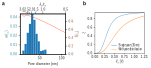
\includegraphics[width=0.9\linewidth]{img/SI-simple-pore-dist.pdf}
   \caption{Salt rejection after considering the pore size
     distribution. \textbf{a}. $w$ (left axis) and $\xi$ (right axis)
     as a function of $r_{\mathrm{G}}$ for the experimental pore size
     distribution with $c_{0}$ = 0.1 mM and $V_{\mathrm{G}}$ = 1.25 V.
     \textbf{b}. Salt rejection ratio $\xi$ as a function of $V_{\mathrm{G}}$ of a
     0.1mM 1:1 salt from a 20 nm-diameter nanopore (blue line) and
     from the experimental pore size distribution (orange line), by
     applying Equation \ref{eq:xi-pore} to main text \Fig{}
     \ref{main-fig:5}b.}
  \label{fig:simple-rect-pore}
\end{figure}

To include the pore size distribution effect for all the salts
studied, we performed FEM analysis for the salt rejection through
single nanopore of different salts with $r_{\mathrm{G}}$ ranges from
2.5 nm to 35 nm, while keeping $c_{0}$ constant at 0.1 mM. As shown in
\Fig{} \ref{fig:xi-salts-pore}, the behavior of $\xi$ vary with the
type of salt. As expected, the overall $\xi$ for monovalent salts
(KCl, NaCl, LiCl) is larger than multivalent salts due to the longer
Debye length. Moreover, $\xi$ of monovalent salts varies less with the
pore size compared with multivalent salts. This can be explained by
the non-linear dependency of $\xi$ on
$\lambda_{\mathrm{D}} / r_{\mathrm{G}}$ as discussed above. Combine
the FEM-simulated $\xi$ values with the experimental pore size
distribution, we obtain main text \Fig{} \ref{main-fig:6}.

\begin{figure}[htbp]
  \centering
   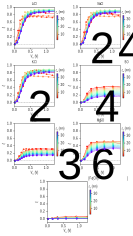
\includegraphics[width=0.75\linewidth]{img/SI-xi-salt-pore-size.pdf}
  \caption{FEM-simulated salt rejction ratio $\xi$ as a function of
    $V_{\mathrm{G}}$ through single nanopores for different salts with
    varied pore radius. All salts have concentration $c_{0}$ = 0.1 mM.}
  \label{fig:xi-salts-pore}
\end{figure}


\pagebreak

\section{Further discussion about the ionic pathway near the graphene pore}
\label{sec:conc}

In this section we provide a more detailed discussion about the
different ionic pathways through the graphene nanopore upon gating in
main text \Fig{} \ref{main-fig:4}b. As disccused in the main text, the
ionic migration is contributed by both diffusion (caused by
concentration gradient) and electrostatic drift (caused by electric
field).  The effect of salt rejection can be viewed as follows: when
$V_{\mathrm{G}}$ = 0, the flux $\boldsymbol{J}_{\mathrm{G}}$ is solely
contributed by the concentration gradient, while after applying a
positive $V_{\mathrm{G}}$, distinct pathways for cations /
anions are created and the drift flux balances the diffusion.

Applying a positive $V_{\mathrm{G}}$ changes the surface distribution
of the cations / anions. To see this, we plot the concentrations of
cation ($c_{+}$) and anion ($c_{-}$) near a graphene nanopore with
$r_{\mathrm{G}}$ = 10 nm, $c_{0}$ = 0.1 mM and $\psi_{\mathrm{G}}$ =
0.15 V, as shown in \Fig{} \ref{fig:conc}a and \ref{fig:conc}b,
respectively. The cations are depleted from the graphene surface,
while the anions are accumulated due to positive
$\psi_{\mathrm{G}}$. The anion concentration at the graphene surface
is enhanced $\sim{}$35 times compared with the bulk concentration in
HCR. The thickness of the depletion / accumulation layer is affected
by the bulk concentration. Here we show this by comparing the radial
distribution of $c_{+}$ and $c_{-}$ along the $z = 0$ line within the
graphene pore. \Fig{} \ref{fig:conc-r} shows such radial ionic
concentration distribution at different $c_{0}$ and $V_{\mathrm{G}}$
levels. When $c_{0}$ = 0.1 mM, $\lambda_{\mathrm{D}}$ is larger than
$r_{\mathrm{G}}$, and the external gate voltage $V_{\mathrm{G}}$ has
control over both $c_{-}$ and $c_{+}$ within the graphene nanopore
(\Fig{} \ref{fig:conc-r}a and \ref{fig:conc-r}c). On the other
hand, when $c_{0}$ = 100 mM, $\lambda_{\mathrm{D}}$ is much smaller
than $r_{\mathrm{G}}$, and the concentration is only affected by
$V_{\mathrm{G}}$ close to the pore edge (\Fig{} \ref{fig:conc-r}b
and \ref{fig:conc-r}d). Therefore by increasing $c_{0}$ (and
equivalently reducing $\lambda_{\mathrm{D}}$), $V_{\mathrm{G}}$ loses
control over the transport in the center of the pore and leads to a
lower $\xi$ value. Due to the existence of graphene quantum
capacitance, the surface potential $\psi_{\mathrm{G}}$ is essentially
smaller than $V_{\mathrm{G}}$, and the maximum surface anion
concentration ($c_{0}$ = 100 mM, $V_{\mathrm{G}}$ = 1.25 V) is
$\sim{}$3 M, much smaller than the saturated surface adsorption
density (at the order of 10$^{2}$ M
\cite{bard_electrochemical_1980}). Therefore we expect the surface
enhancement of the anions under the FEM conditions to be realistic and
the influence of the anion concentration on the diffusivity is minimal
\cite{Tang_1999_I}.


\begin{figure}[htbp]
  \centering
  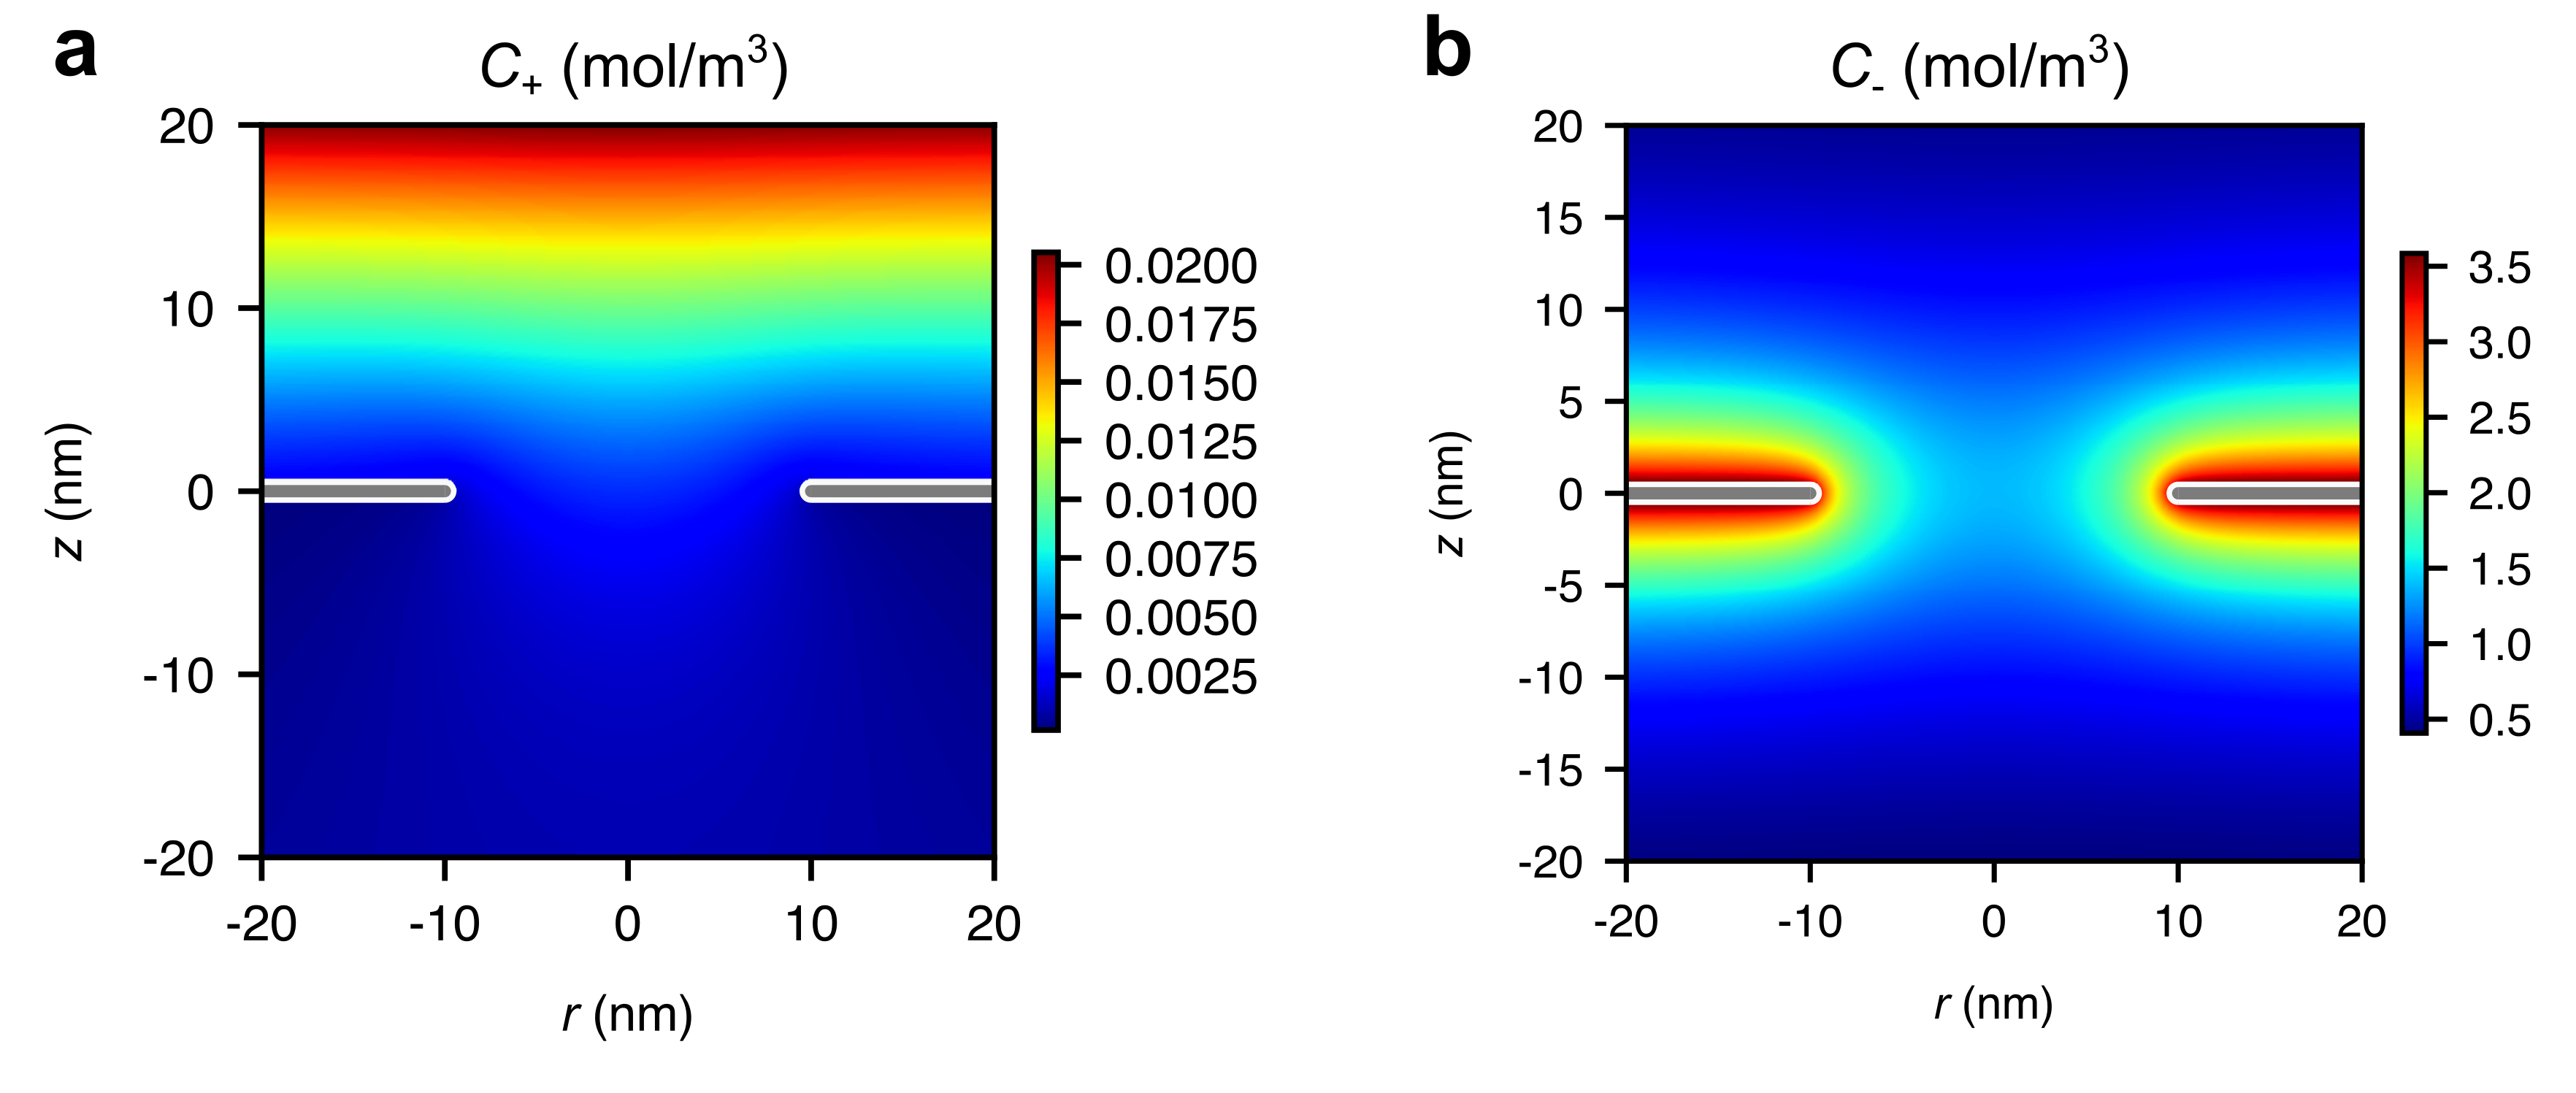
\includegraphics[width=0.8\linewidth]{img/SI-concentration.pdf}
  \caption{Cation concentration $c_{+}$ (\textbf{a}.) and anion
    concentration $c_{-}$ (\textbf{b}.) near the graphene nanopore
    with $r_{\mathrm{G}}$ = 10 nm, $c_{0}$ = 0.1 mM, and
    $\psi_{\mathrm{G}}$ = 0.15 V, for a KCl solution at 0.1
    mM. Depletion of cation and accumulation of anion can be observed
    near the graphene surface.}
  \label{fig:conc}
\end{figure}

\begin{figure}[htbp]
  \centering
  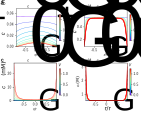
\includegraphics[width=0.75\linewidth]{img/SI-conc-r.pdf}
  \caption{Radial distribution of ions along the line $z=0$ within a
    graphene nanopore with $r_{\mathrm{G}}$ = 10 nm: (\textbf{a}.)
    $c_{+}$ at $c_{0}$ = 0.1 mM, (\textbf{b}.) $c_{+}$ at $c_{0}$ =
    100 mM, (\textbf{c}.) $c_{-}$ at $c_{0}$ = 0.1 mM and
    (\textbf{d}.) $c_{-}$ at $c_{0}$ = 100 mM. The lines with varied
    colors indicate the difference of $V_{\mathrm{G}}$ applied.}
  \label{fig:conc-r}
\end{figure}

Next we analyze the diffusion and drift contributions to the ionic
transport. As shown in \Fig{} \ref{fig:potential}, the
electrochemical potential energy $\mu_{i}$ is decomposed into the
electric potential energy $z_{i} c_{i} \psi_{i}$ (\Fig{}
\ref{fig:potential}a and \ref{fig:potential}b) and the chemical
potential energy $k_{\mathrm{B}}T \ln x_{i}$ (\Fig{}
\ref{fig:potential}c and \ref{fig:potential}d) near a graphene
nanopore with $r_{\mathrm{G}}$ = 10 nm and $\psi_{\mathrm{G}}$ = 0.15
V. The transport of cations is dominated by its chemical potential and
the diffusion is prominent in the center of the pore. On the other
hand, the electric and diffusive potential energies are similar with
opposite signs and counterbalance each other. This explains the
relatively smaller electrochemical potential of anions in main text
\Fig{} \ref{main-fig:4}b. As a result, different pathways for cations
and anions emerge that cations preferably pass through the pore
center, while anions mainly pass near the pore edge, as shown in
\Fig{} \ref{fig:flux}.

\begin{figure}[htbp]
  \centering
  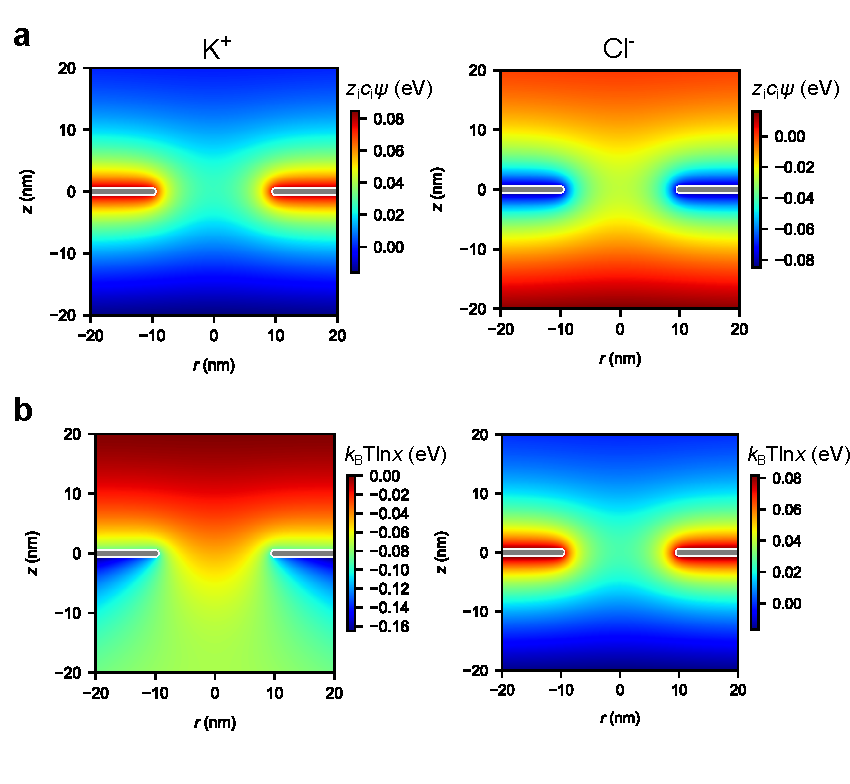
\includegraphics[width=0.8\linewidth]{img/SI-electrochemical-decomposite.pdf}
  \caption{Decomposition of electrochemical potential near a nanopore
    corresponding to main text \Fig \ref{main-fig:4}. \textbf{a}. The electrostatic
    (drift) contribution to the electrochemical potential for cation
    (left) and anion (right) and \textbf{b}. The concentration (diffusion)
    contribution to the electrochemical potential for cation (left)
    and anion (right). The relative small order of magnitude for anion
    electrochemical potential is caused by the balance between the
    diffusion and drift for anion.}
  \label{fig:potential}
\end{figure}

\begin{figure}[htbp]
  \centering
  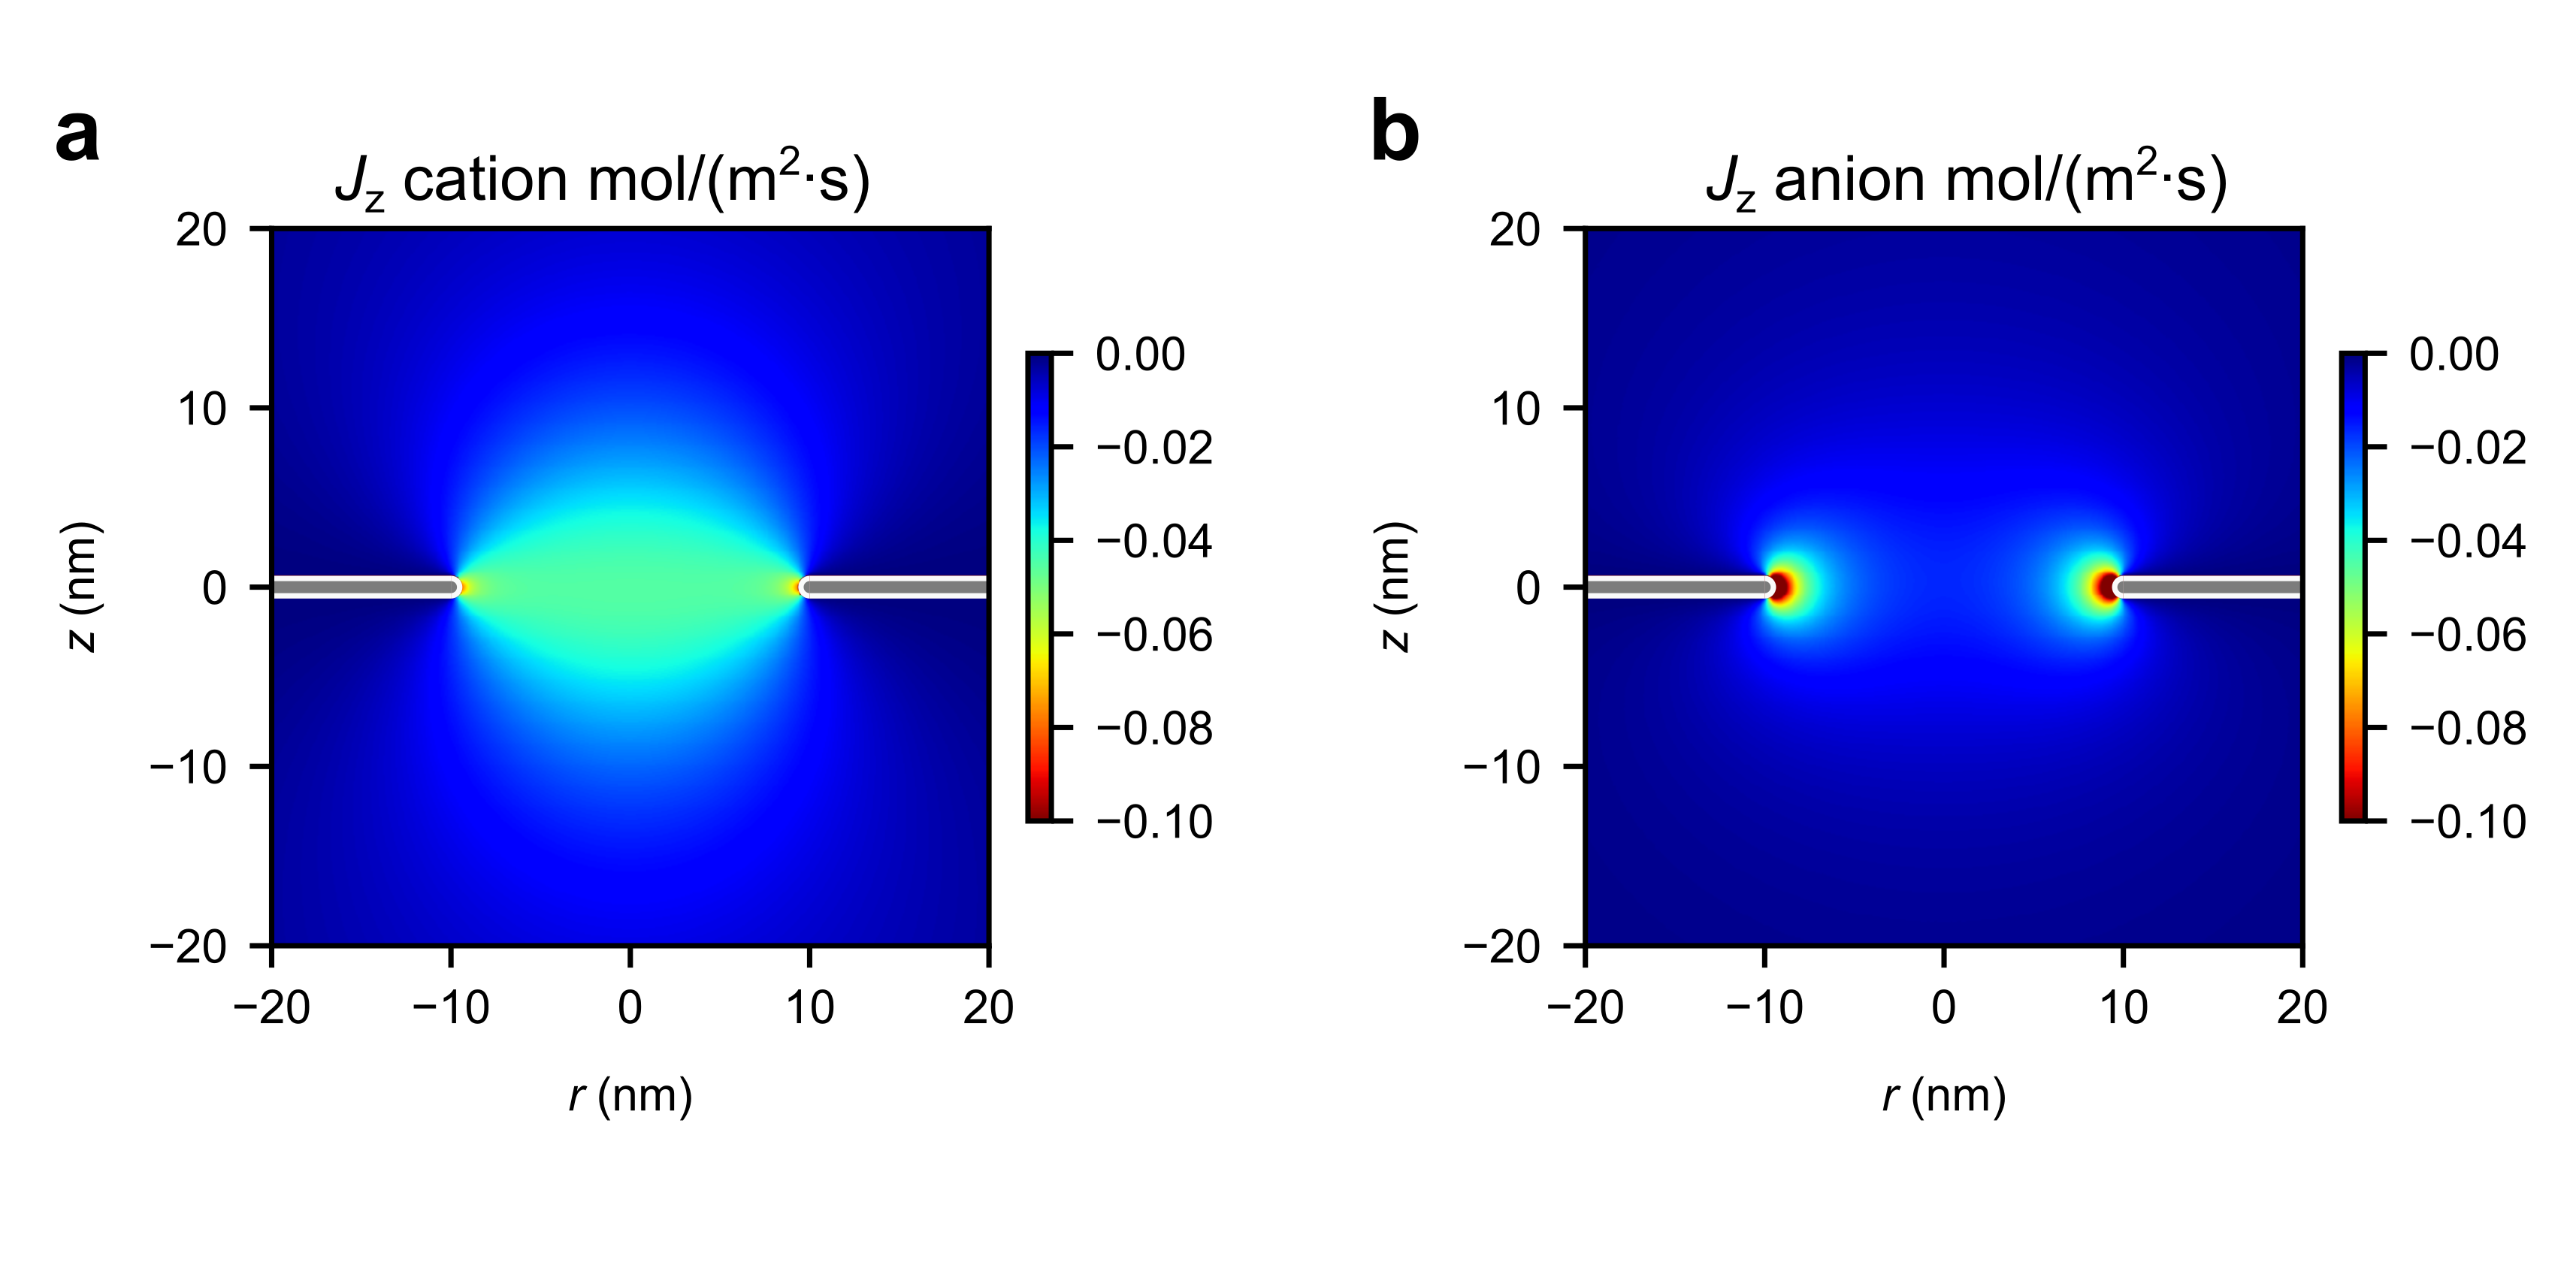
\includegraphics[width=0.8\linewidth]{img/SI-flux.png}
  \caption{z-component fluxes of cation ($J_{z+}$, \textbf{a}.)  and
    anion ($J_{z-}$ \textbf{b}.) near the graphene nanopore
    corresponding to \Fig{} \ref{main-fig:4}b in main text. The
    pathways for the different ions can be spatially distinguished:
    the flux of cation passes mostly through the center of the
    graphene nanopore while the anion passes mainly through the
    edge. The analysis is in consistent with the gradient of chemical
    potential as shown in the main text \Fig{} \ref{main-fig:4}b.}
  \label{fig:flux}
\end{figure}

We note that when the surface potential $\psi_{\mathrm{G}}$ of
graphene further increases, the salt rejection may be weakened, or
even enhanced salt transport is observed. To see this we artificially
increase the $\psi_{\mathrm{G}}$ up to over 1 V when not considering
the limiting effect of graphene quantum capacitance. As seen in \Fig{}
\ref{fig:reverse}, for each salt concentration $c_{0}$, the averaged
total flux $J_{z}$ does not further decrease when $\psi_{\mathrm{G}}$
is larger than a critical potential $V_{\mathrm{c}}$. At low $c_{0}$,
further increasing $\psi_{\mathrm{G}}$ over $V_{\mathrm{c}}$ may even
enhance the flux, leading to a negative $\xi$. The reserve of the salt
rejection at higher $V_{\mathrm{G}}$ values is caused by the enhanced
anion flux around the pore edge, while the cation flux saturates
(\Fig{} \ref{fig:large-V}). Such flux enhancement resemble that in an
ionic transistor \cite{Nam_2009,Cheng_2018} when ionic current rises
by applying gate voltage. Nevertheless, such regime may not be easy to
be observed experimentally as the $V_{\mathrm{G}}$ applied may already
exceed the electrochemical window of water, due to the quantum
capacitance of graphene.

\begin{figure}[htbp]
  \centering
  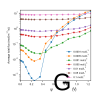
\includegraphics[width=0.5\linewidth]{img/SI-rect-reverse.pdf}
  \caption{Average total flux $J_{z}$ in the nanopore as
    a function of $\psi_{\mathrm{G}}$ at different concentrations. The
    range of $\psi_{\mathrm{G}}$ is larger than the experimentally
    achievable value. The rectification of flux becomes weaker after a
    certain level of $\psi_{\mathrm{G}}$ is reached. Further
    increasing the surface potential of graphene may even enhance the
    transportation of ions, which is similar to the cases of ionic
    transistors.}
  \label{fig:reverse}
\end{figure}


\begin{figure}[htbp]
  \centering
  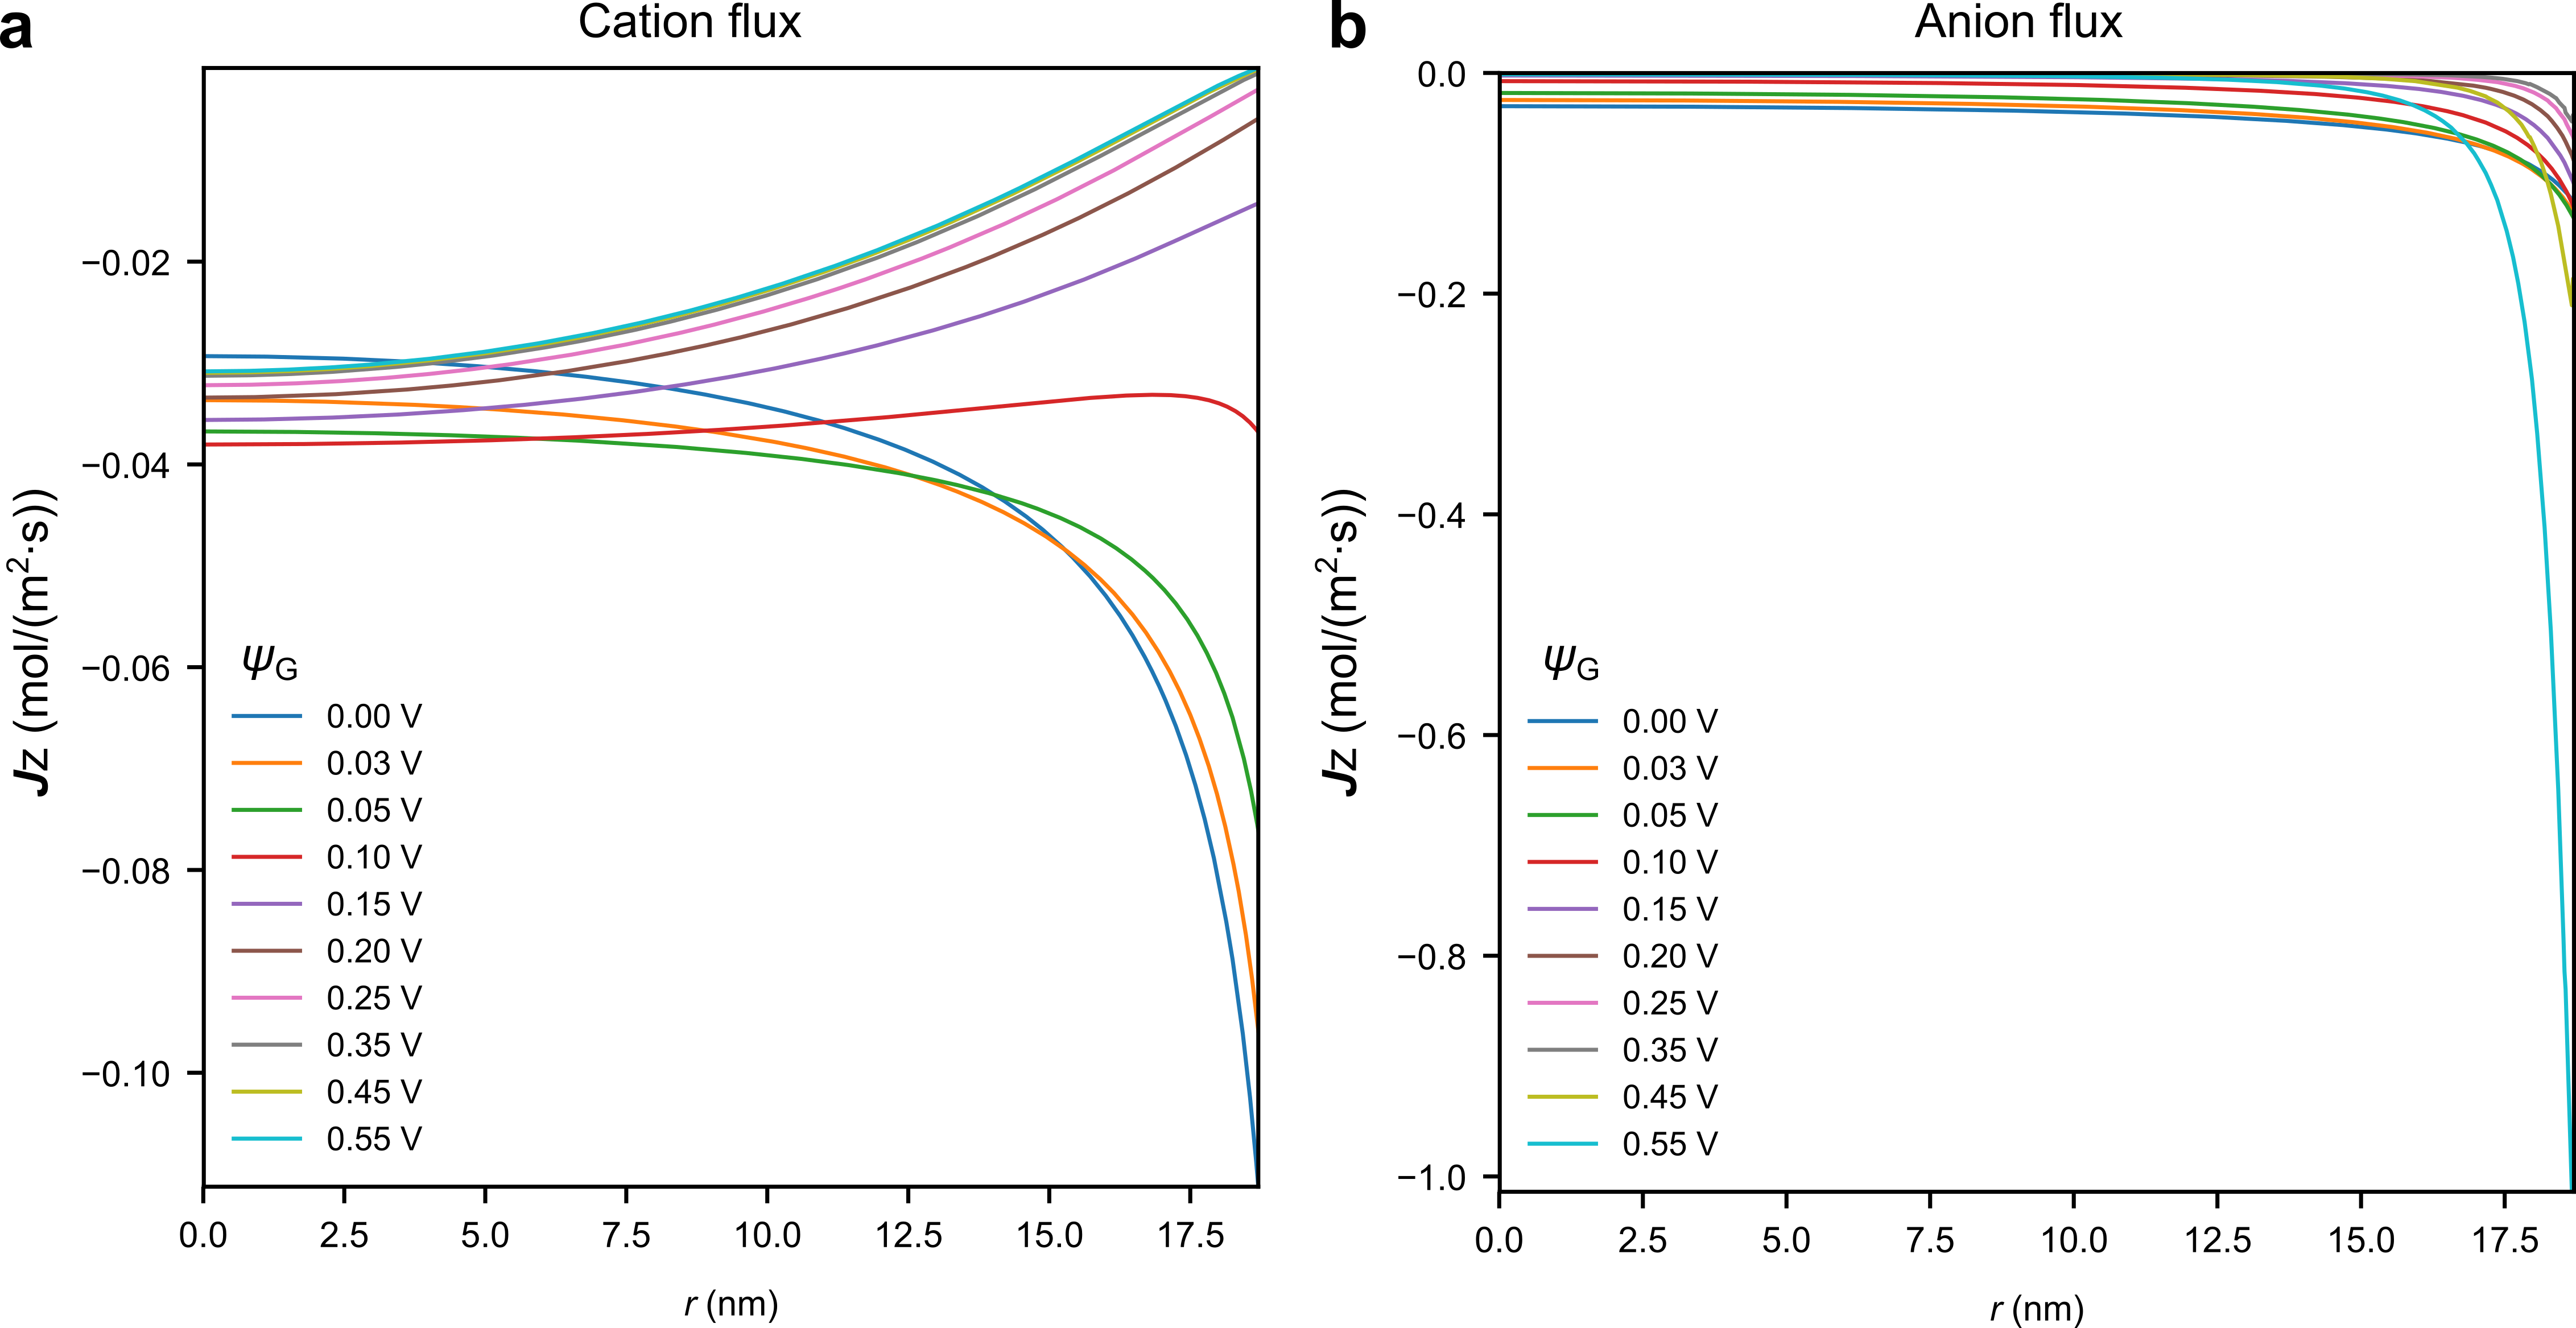
\includegraphics[width=0.8\linewidth]{img/SI-flux-larger.png}
  \caption{Spatial distribution of $J_{z}$ at $z = 0$ as a function
    of $r$ in a nanopore with $r_{\mathrm{G}}$ = 20 nm, at different
    levels of $\psi_{\mathrm{G}}$ (larger than experimentally
    achievable values) for cation (\textbf{a}.) and anion
    (\textbf{b}.). The cation flux becomes nearly saturated with
    increasing $\psi_{\mathrm{G}}$, while the flow of anion near the
    pore edge becomes much larger. The drastic increase of
    pore-bounded anion flux is caused by the accumulation of anions
    near the graphene surface, and in turn causes the increasing of
    total flux as seen in \Fig \ref{fig:reverse}.}
  \label{fig:large-V}
\end{figure}
\clearpage{}


\section{Further details of the numerical simulation }
\label{sec:numer}

The numerical simulations were carried out using COMSOL Multiphysics
5.3a. The simulation domain is shown in \Fig \ref{fig:scheme}. To
simplify the geometry, we use axial symmetric coordinate system. The
radius \textit{L} and height \textit{H} of both HCR and LCR are set to
20 $r_{\mathrm{G}}$, the radius of the nanopore. The potential at the
bottom of the LCR and the center of the graphene domains are set to be
0 and $\psi_{\mathrm{G}}$, respectively. The potential at the end of
HCR is not set explicitly, but rather determined through the Poisson
equation with no flux boundary condition
$\boldsymbol{D}^{\mathrm{norm}}=0$. The relative permittivity in the
HCR and LCR is set as $\varepsilon_{\mathrm{}}=78$. The relative
permittivity of the Stern layer is set to
$\varepsilon_{\mathrm{H}}=20$\cite{Conway_1951} and for the graphene
domain we set the relative permittivity as a large number
(e.g. $10^{5}$) for a better convergence of the solver.  For the
transport of diluted ionic species, we use the PNP equations to
describe the diffusion and drift of the ions, which can be further
unified by the gradient of electrochemical potential, as described in
the main text. The initial values of the electrolyte is set to $c_{0}$
in HCR and 0.1 $c_{0}$ in LCR. At the ends of the cells in the
z-direction, we use the inlet boundaries conditions for the
concentration of electrolytes, that the concentration on these
boundaries remains the same with the initial value, due to the
effective mixing in the experimental setup.

\begin{figure}[htbp]
  \centering
  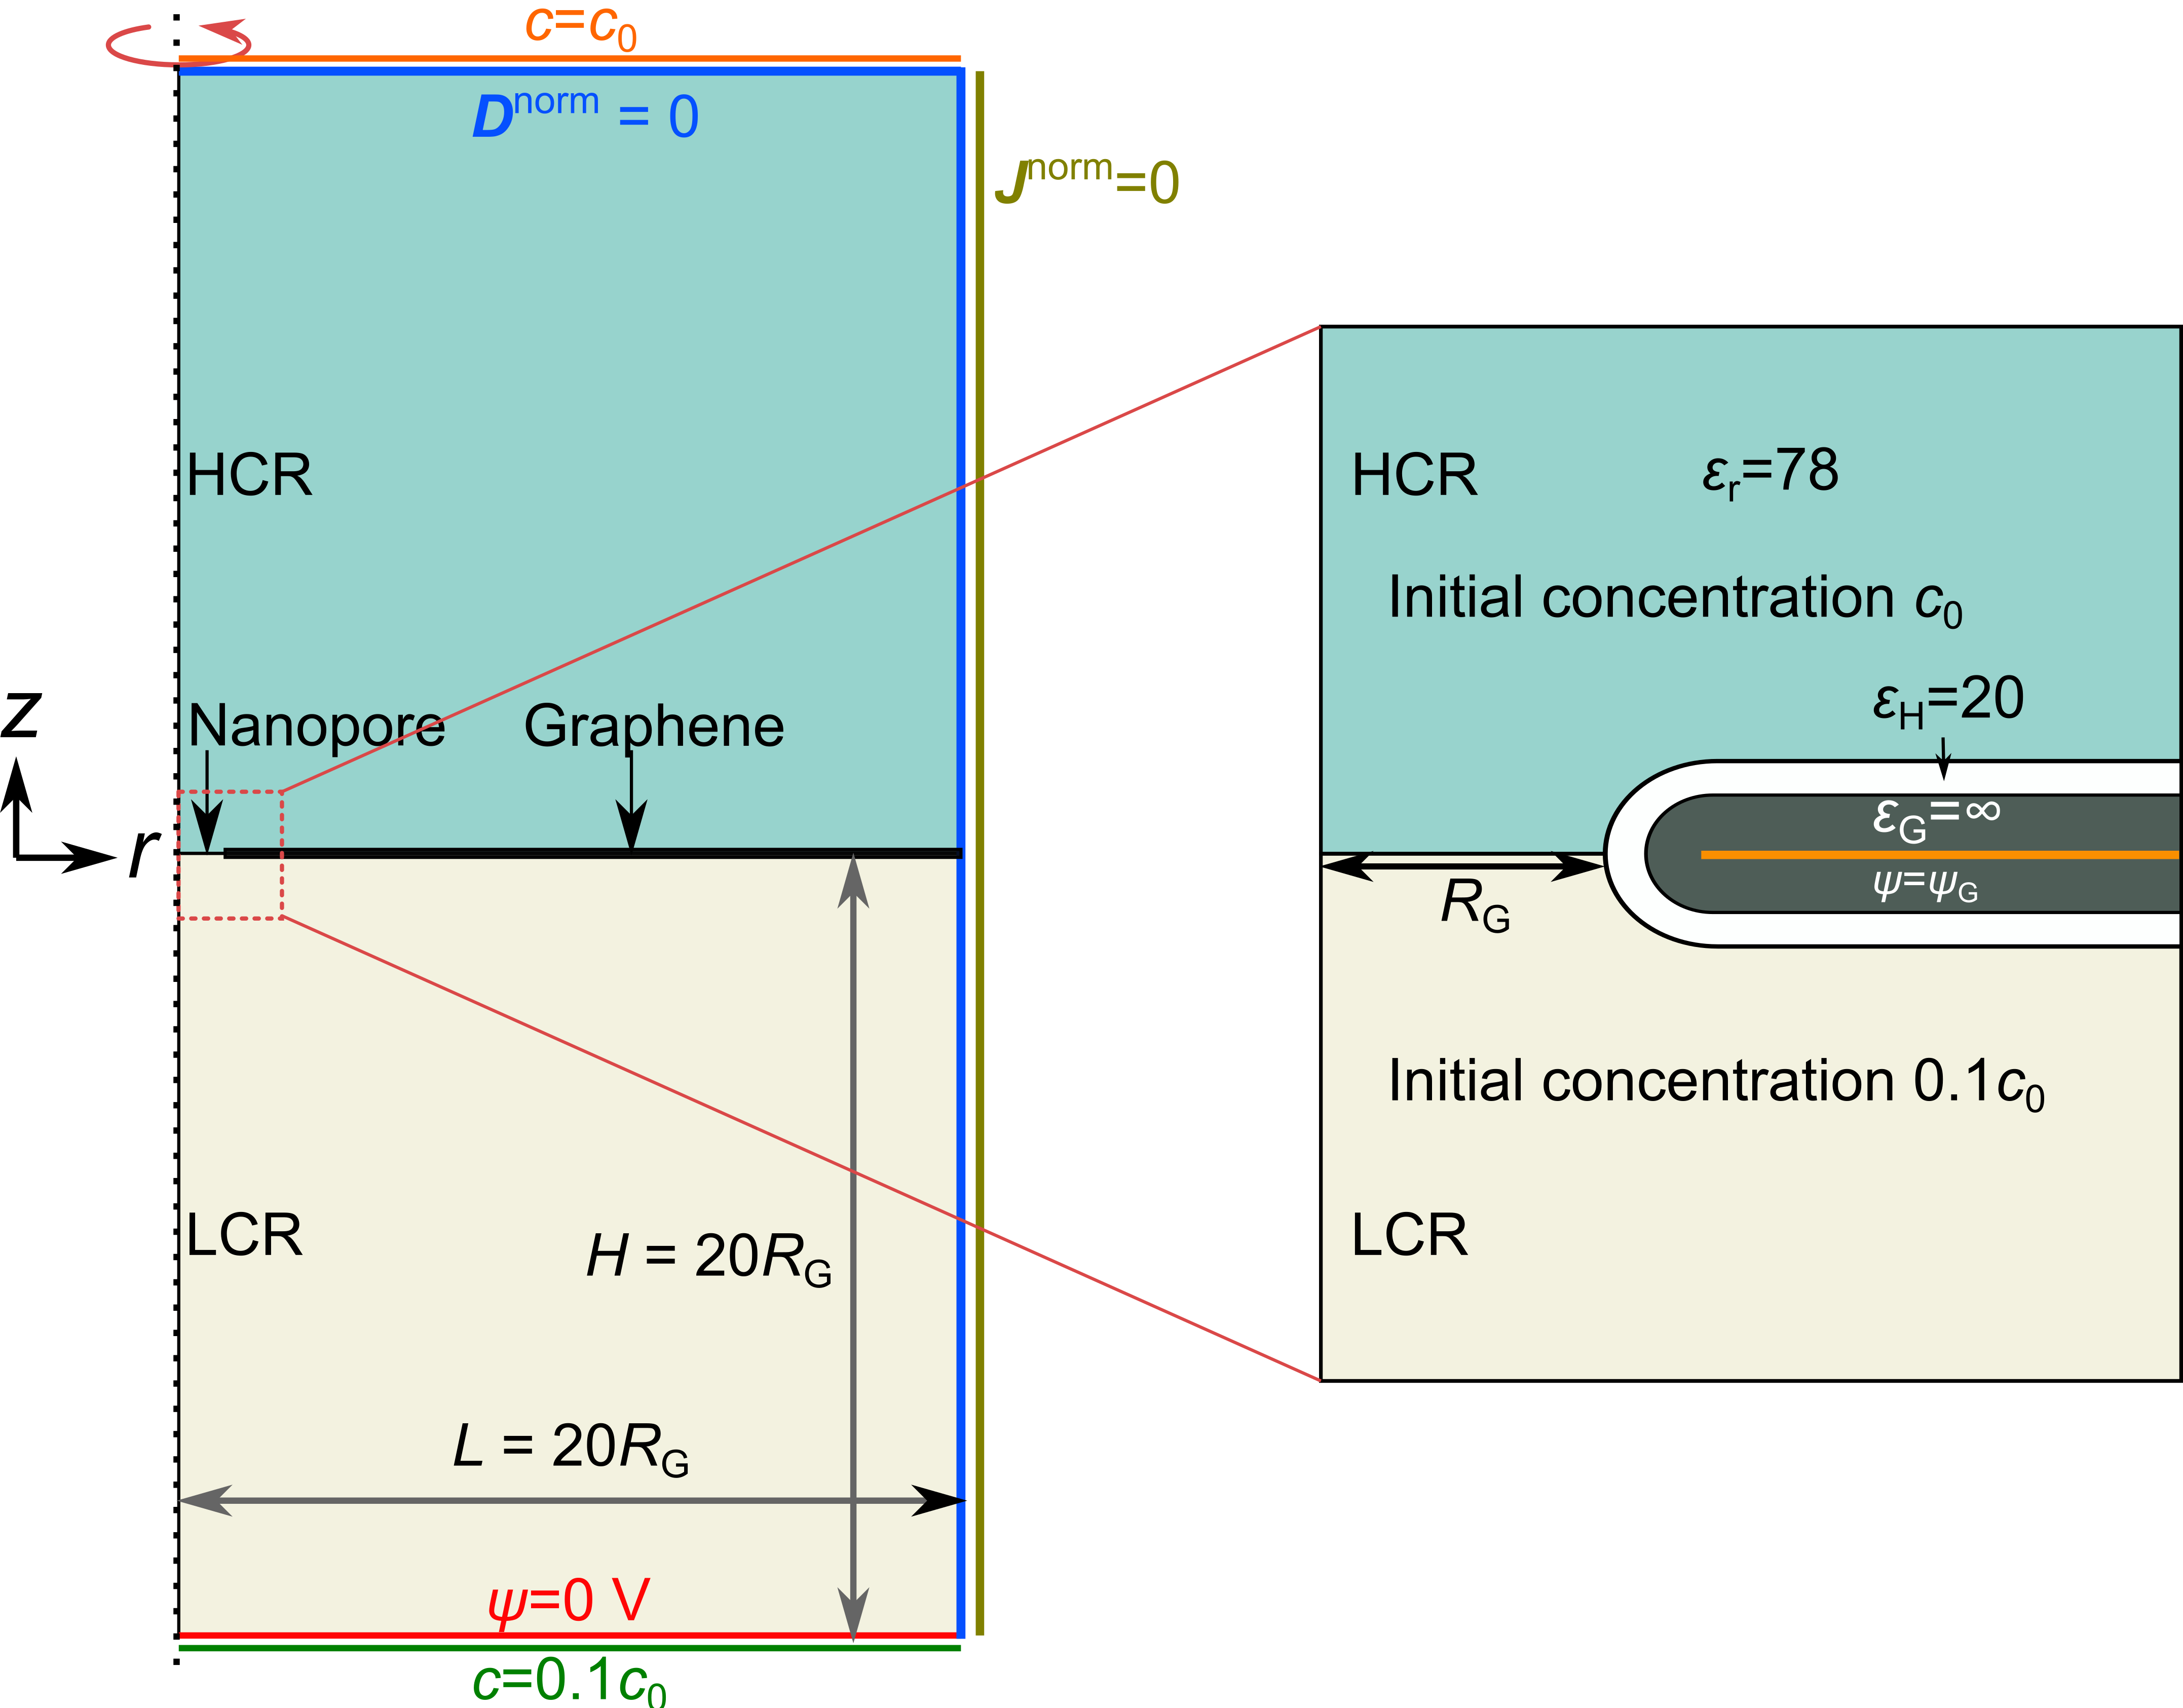
\includegraphics[width=0.8\linewidth]{img/SI-numerical-1.png}
  \caption{Scheme of the simulation domain used. Left: geometry of the
    whole simulation domain. Right: configuration near the graphene
    nanopore, corresponding to the red rectangle on the left side.}
  \label{fig:scheme}
\end{figure}

The transport of ionic species is described by the steady-state
Nernst-Planck equation:
\begin{eqnarray}
  \label{eq:pnp}
  \nabla \cdot \boldsymbol{J}_{i} = -\nabla \cdot \left( \frac{D_{i}}{k_{\mathrm{B}}T} c_{i} N_{\mathrm{A}} \nabla \mu_{i}\right)
  = -\nabla \cdot \left( \frac{D_{i}}{k_{\mathrm{B}} T} c_{i} N_{\mathrm{A}}
  [k_{\mathrm{B}}T \nabla \ln x_{i} + z_{i} e \nabla \psi]\right) = 0\\
  x_{i} = \frac{c_{i}}{\sum_{i} c_{i} + c_{\mathrm{H_{2}O}}}
\end{eqnarray}
The potential distribution within the whole simulation domain is
described by the Poisson equation:
\begin{equation}
  \label{eq:poisson}
  \nabla \cdot (\varepsilon_{\mathrm{m}} \varepsilon_{0} \nabla \psi) = -N_{\mathrm{A}} e \sum_{i} c_{i}z_{i}
\end{equation}
Where $\varepsilon_{\mathrm{m}}$ is the relative permittivity of
domain m. The contribution of mobile charges is only valid in the
solution domain. The use of a large $\varepsilon_{\mathrm{G}}$ ensures
that the potential in the whole simulation domain can be solved
continuously. 

To simulate the applied external bias $V_{\mathrm{G}}$, we set the
value of $\psi_{\mathrm{G}}$ explicitly and extract the charge
$\sigma_{\mathrm{G}}$ by:
\begin{equation}
  \label{eq:sigma-G}
  \sigma_{\mathrm{G}} = - {\displaystyle \frac{\int_{\mathrm{\Omega}} z_{i} c_{i} N_{\mathrm{A}} e \mathrm{d}^{3} \Omega}{S_{\mathrm{G}}}}
\end{equation}
and $V_{\mathrm{G}}$ is then calculated by:
\begin{eqnarray}
  \label{eq:VG}
  V_{\mathrm{G}} = \Delta \phi_{\mathrm{G}} + \psi_{\mathrm{G}}\\
  \sigma_{\mathrm{G}} = \int_{0}^{\Delta \phi_{\mathrm{G}}} \frac{1}{C_{\mathrm{Q}}(\phi_{\mathrm{G}})} \mathrm{d} \phi_{\mathrm{G}}
\end{eqnarray}
where the quantum capacitance
$C_{\mathrm{Q}}=\partial \sigma_{\mathrm{G}}/\partial
\phi_{\mathrm{G}}$ is calculated by Eq. 8 in main text.

\begin{figure}[htbp]
  \centering
  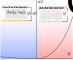
\includegraphics[width=0.5\linewidth]{img/SI-trap.png}
  \caption{Schematic illustration of the origin of the asymmetric
    rectification with respect to $V_{\mathrm{G}}$. Due to the
    existence of surface charge traps at negative $V_{\mathrm{G}}$,
    the graphene is less charged compared to the positive
    $V_{\mathrm{G}}$.}
  \label{fig:trap}
\end{figure}

Note that due to the existence of electron traps on graphene due to
fabrication process, the induced charge traps on graphene effectively
reduce the charge density on graphene and greatly attenuate the
surface potential on graphene, as illustrated in \Fig
\ref{fig:trap}. This effect is universally observed in
CVD-graphene-based field effect transistors in air, while the
mechanism is fully understood yet. In view of this, we only simulate
the situation where $V_{\mathrm{G}}>$ 0 for the salt rejection
mechanism. The trend that $\xi$ is almost independent of
$V_{\mathrm{G}}$ when $V_{\mathrm{G}}<$ 0 can be qualitatively
explained by the existence of surface charge traps as stated above.
We have also tested the mesh-independence of our solutions. As show in
in \Fig{} \ref{fig:mesh}a, we use two parameters to control the
refinement of the mesh entities: (i) triangle mesh division
$N_{\mathrm{div}}$, giving the smallest triangle mesh size
$\delta_{\mathrm{G}} / N_{\mathrm{div}}$, where $\delta_{\mathrm{G}}$
is the thickness of graphene, and (ii) division of mesh
$N_{\mathrm{b}}$, on the boundary $0<r<r_{\mathrm{G}};z=0$. The
solution convergence is evaluated by the mean absolute error (MAE) of
anion flux $\boldsymbol{J}_{z}$ on the boundary
$0<r<r_{\mathrm{G}};z=0$, as shown in \Fig{}
\ref{fig:mesh}b. The solution of the PNP model is sensitive to the
value $N_{\mathrm{b}}$, and can be regarded numerically converged when
$N_{\mathrm{b}}>100$. Combining the calculation effort and numerical
precision, we adapt the value $N_{\mathrm{div}}=5$ and
$N_{\mathrm{b}}=100$ in our simulations.

\begin{figure}[htbp]
  \centering
  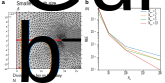
\includegraphics[width=0.8\linewidth]{img/SI-mesh.pdf}
  \caption{Mesh independence of the solution. \textbf{a}. Scheme of
    the mesh refinement near the graphene pore. The values
    $N_{\mathrm{div}}$ and $N_{\mathrm{b}}$ controls the size of mesh
    along the boundary $z=0, 0<r<r_{\mathrm{G}}$ (shown in
    red). \textbf{b}. Mean absolute error (MAE) of the anion flux
    $\boldsymbol{J}_{z}$ along the boundary $z=0,
    0<r<r_{\mathrm{G}}$. The error is more sensitive to
    $N_{\mathrm{b}}$ than $N_{\mathrm{div}}$.}
  \label{fig:mesh}
\end{figure}

\section{Conductivity and Debye length for all salts}
\label{sec:salts}
In Table \ref{tab:conductivity}, the conductivities and calculated Debye
lengths for 6 salts are shown. At the same concentration, the higher
ionic strength of the multivalent salts leads to a reduction of the
respective Debye lengths.

\begin{table}[htbp]
  \centering
  \begin{tabular}{lcc}
    \hline
    Solution & Conductivity (mS$\cdot$cm$^{-1}$) & $\lambda_{\mathrm{D}}$ (nm) \\
    \hline
    0.1 mM NaCl &1.80$\times$10$^{-2}$  &30.4\\
    0.1 mM LiCl &1.58$\times$10$^{-2}$ &30.4\\
    0.1 mM CaCl$_{2}$&  2.19$\times$10$^{-2}$ &17.2\\
    0.1 mM MgSO$_{4}$   &3.27$\times$10$^{-2}$ &15.2\\
    0.1 mM K$_{2}$SO$_{4}$      &4.16$\times$10$^{-2}$ &17.2\\
    0.1 mM K$_{3}$[Fe(CN)$_{6}$]&       5.95$\times$10$^{-2}$  &12.4\\
    \hline
  \end{tabular}
  \caption{Conductivity and $\lambda_{\mathrm{D}}$ of various salts.}
  \label{tab:conductivity}
\end{table}


\section*{}
\label{sec:ref}
\bibliography{ref}

\end{document}
